% if you need to pass options to natbib, use, e.g.:
% \PassOptionsToPackage{numbers, compress}{natbib}
% before loading nips_2016
%
% to avoid loading the natbib package, add option nonatbib:
% \usepackage[nonatbib]{nips_2016}

\usepackage[nonatbib]{nips_2016}

% to compile a camera-ready version, add the [final] option, e.g.:
% \usepackage[final]{nips_2016}

\usepackage[utf8]{inputenc} % allow utf-8 input
\usepackage[T1]{fontenc}    % use 8-bit T1 fonts
\usepackage{hyperref}       % hyperlinks
\usepackage{url}            % simple URL typesetting
\usepackage{booktabs}       % professional-quality tables
\usepackage{amsfonts}       % blackboard math symbols
\usepackage{nicefrac}       % compact symbols for 1/2, etc.
\usepackage{microtype}      % microtypography
% \usepackage{fullpage,subfigure,fancyhdr}
\usepackage[pdftex]{color}
\usepackage{wrapfig}
% \usepackage{textcomp}
% \usepackage{verbatim}
% \usepackage{times}
\usepackage{amsmath,amssymb,amsthm}	% math equations, symbols, theorems
\usepackage{mdwlist}	% list-related commands
\usepackage{subfigure}	% subfigures
\usepackage{sidecap}
\usepackage{wrapfig}
\usepackage{xspace}
\usepackage{algorithm,algorithmicx}
\usepackage{algcompatible}
\usepackage[pdftex]{graphicx}
% \usepackage[sort&compress,comma,round,numbers]{natbib}
\usepackage{pict2e}
\usepackage[nottoc,numbib]{tocbibind}
\usepackage{paralist}
\usepackage{multicol}
\usepackage{lettrine}
\usepackage{caption}
\usepackage{helvet}

%%%%%%%%% COMMENTS %%%%%%%%%
\newcommand{\jv}[1]{{\color{magenta}{#1}}}

%%%%%%%%% MATH OPERATORS %%%%%%%%%%%%
\providecommand{\ve}[1]{\boldsymbol{#1}}
\providecommand{\ma}[1]{\boldsymbol{#1}}
\providecommand{\norm}[1]{\left \lVert#1 \right  \rVert}
\providecommand{\deter}[1]{\lvert #1 \rvert}
\providecommand{\abs}[1]{\left \lvert #1 \right \rvert}
\providecommand{\mat}[1]{\left[ #1 \right]}
\newcommand{\trans}[1]{{#1}^{\ensuremath{\mathsf{T}}}}           % transpose
\newcommand{\transpose}[1]{{#1}^{\ensuremath{\mathsf{T}}}}           % transpose
\newcommand{\argmax}{\operatornamewithlimits{argmax}}
\newcommand{\argmin}{\operatornamewithlimits{argmin}}
\newcommand{\T}{^{\ensuremath{\mathsf{T}}}}           % transpose
\newcommand{\from}{{\ensuremath{\colon}}}           % :
\newcommand{\trace}[1]{{\ensuremath{\operatorname{tr}\!\left(#1\right)}}}           % :

\providecommand{\ms}[1]{\mathsf{#1}}
\providecommand{\mc}[1]{\mathcal{#1}}
\providecommand{\mt}[1]{\widetilde{#1}}
\providecommand{\mb}[1]{\boldsymbol{#1}}
\providecommand{\mbb}[1]{\mathbb{#1}}
\providecommand{\mv}[1]{\vec{#1}}
\providecommand{\mh}[1]{\hat{#1}}
\providecommand{\wh}[1]{\widehat{#1}}
\providecommand{\mhv}[1]{\mh{\mv{#1}}}
\providecommand{\mvh}[1]{\mv{\mh{#1}}}
\providecommand{\mhc}[1]{\hat{\mathcal{#1}}}
\providecommand{\mbc}[1]{\mb{\mathcal{#1}}}
\providecommand{\mvc}[1]{\mv{\mathcal{#1}}}
\providecommand{\mtc}[1]{\widetilde{\mathcal{#1}}}
\providecommand{\mth}[1]{\mt{\mh{#1}}}
\providecommand{\mht}[1]{\mh{\mt{#1}}}
\providecommand{\mhb}[1]{\hat{\boldsymbol{#1}}}
\providecommand{\whb}[1]{\widehat{\boldsymbol{#1}}}
\providecommand{\mvb}[1]{\vec{\boldsymbol{#1}}}
\providecommand{\mtb}[1]{\widetilde{\boldsymbol{#1}}}
\providecommand{\mbt}[1]{\widetilde{\boldsymbol{#1}}}
\providecommand{\mvc}[1]{\vec{\mathcal{#1}}}
% \newcommand{\D}[2]{\frac{\partial #1}{\partial #2}}
\newcommand{\dd}[2]{\frac{\partial ^2 #1}{\partial #2 ^2}}
\newcommand{\DDD}[3]{\frac{\partial ^2 #1}{\partial #2 \partial #3}}
\newcommand{\Di}[2]{\frac{\partial ^i #1}{\partial #2 ^i}}

%%%%%% SHORT HAND %%%%%%%%%%
\renewcommand{\refname}{References and Notes}

\newcommand{\Vr}{V_{reset}}
\newcommand{\Vl}{V_{leat}}
\newcommand{\eqdef}{\overset{\triangle}{=}}
\newcommand{\grad}{\nabla}
\newcommand{\Hess}{\nabla\nabla}
\newcommand{\defn}{\overset{\triangle}{=}}

\newcommand{\iid}{\overset{iid}{\sim}}
\newcommand{\knn}{$k$NN}

\newcommand{\elegans}{\emph{C. elegans} }

\newcommand{\Lik}{\mathcal{L}}
\newcommand{\Cae}{[\widehat{\text{Ca}}^{2+}]}
\newcommand{\Cav}{\ve{C}}%[\ve{\text{Ca}}^{2+}]}
\newcommand{\sml}{\sqrt{\ma{\lambda}}}
\newcommand{\ml}{\ma{\lambda}}
\newcommand{\nw}{\widehat{n}}
\newcommand{\nv}{\vec{n}}
\newcommand{\Ae}{\widehat{A}}
\newcommand{\te}{\widehat{\tau}}
\newcommand{\maxn}{\max_{\ve{n}: n_t \geq 0}}
% \newcommand{\V}{\text{Var}}

\newcommand{\PmcP}{P \in \mc{P}}
\newcommand{\mP}{\mathbb{P}}

% \newcommand{\dvs}{\dot{\bs}_t}
% \newcommand{\dvw}{\dot{\bw}_t}
% \newcommand{\dvx}{\dot{\bx}_t}
% \newcommand{\dvy}{\dot{\by}_t}

\newcommand{\ft}{f_{\ve{\thet}}}
\newcommand{\gt}{g_{\ve{\thet}}}
\newcommand{\hht}{h_{\thetn}}

\newcommand{\Real}{\mathbb{R}}


\newcommand{\wconv}{\overset{i.p.}{\rightarrow}}
\newcommand{\sconv}{\overset{i.p.}{\rightarrow}}
\newcommand{\conv}{\rightarrow}
\newcommand{\pconv}{\overset{p}{\conv}}
\newcommand{\mcE}{\mathcal{E}}
\newcommand{\mcT}{\mathcal{T}}
\newcommand{\mcG}{\mathcal{G}}
\newcommand{\mcM}{\mathcal{M}}
\newcommand{\mcL}{\mathcal{L}}
\newcommand{\hatmcE}{\widehat{\mcE}}
\newcommand{\hatp}{\widehat{p}}
\newcommand{\hatP}{\widehat{P}}
\newcommand{\hatQ}{\widehat{Q}}
\newcommand{\hatL}{\widehat{L}}
\newcommand{\mhP}{\widehat{\PP}}
\newcommand{\tildeA}{\widetilde{A}}
\newcommand{\defeq}{\overset{\triangle}{=}}


\DeclareMathOperator{\Pmat}{\mathbf{P}}
\DeclareMathOperator{\veta}{\mathbf{\mb{v}}}
\DeclareMathOperator*{\minimize}{\mathrm{minimize}}
\DeclareMathOperator*{\maximize}{\mathrm{maximize}}
% \DeclareMathOperator*{\mb{v}mod}{\mathbf{\mb{v}}}


%%%%%%% LATIN LETTERS


\newcommand{\bA}{\mb{A}}
\newcommand{\bB}{\mb{B}}
\newcommand{\bD}{\mb{D}}
\newcommand{\bE}{\mb{E}}
\newcommand{\bI}{\mb{I}}
\newcommand{\bP}{\mb{P}}
\newcommand{\bS}{\mb{S}}
\newcommand{\bU}{\mb{U}}
\newcommand{\bV}{\mb{V}}
\newcommand{\bW}{\mb{W}}
\newcommand{\bX}{\mb{X}}
\newcommand{\bY}{\mb{Y}}
\newcommand{\bZ}{\mb{Z}}

\newcommand{\ba}{\mb{a}}
\renewcommand{\ba}{\mb{b}}
\newcommand{\bd}{\mb{d}}
\newcommand{\be}{\mb{e}}
\newcommand{\bp}{\mb{p}}
\newcommand{\bs}{\mb{s}}
\newcommand{\bu}{\mb{u}}
\newcommand{\bv}{\mb{v}}
\newcommand{\bw}{\mb{w}}
\newcommand{\bx}{\mb{x}}
\newcommand{\by}{\mb{y}}
\newcommand{\bz}{\mb{z}}


\newcommand{\Aa}{\mathbb{A}}
\newcommand{\BB}{\mathbb{B}}
\newcommand{\CC}{\mathbb{C}}         
\newcommand{\DD}{\mathbb{D}}         
\newcommand{\EE}{\mathbb{E}}           % expected value
\newcommand{\FF}{\mathbb{F}}         
\newcommand{\GG}{\mathbb{G}}
\newcommand{\HH}{\mathbb{H}}         
\newcommand{\II}{\mathbb{I}}           % indicator function
\newcommand{\LL}{\mathbb{L}}
\newcommand{\MM}{\mathbb{M}}
\newcommand{\NN}{\mathbb{N}}
\newcommand{\PP}{\mathbb{P}}         
\newcommand{\QQ}{\mathbb{Q}}           
\newcommand{\SSS}{\mathbb{S}}           
\newcommand{\VV}{\mathbb{V}}
\newcommand{\WW}{\mathbb{W}}         
\newcommand{\XX}{\mathbb{X}}         
\newcommand{\YY}{\mathbb{Y}}
\newcommand{\ZZ}{\mathbb{Z}}         




\newcommand{\Qs}{Q}
\newcommand{\mcS}{\mc{S}}
\newcommand{\mcU}{\mc{U}}

\newcommand{\mbd}{\mb{d}}
\newcommand{\mbD}{\mb{D}}
\newcommand{\mbx}{\mb{x}}
\newcommand{\mbX}{\mb{X}}
\newcommand{\mby}{\mb{y}}
\newcommand{\mbY}{\mb{Y}}

\newcommand{\mtbd}{\mtb{d}}
\newcommand{\mtbD}{\mtb{D}}
\newcommand{\mtbx}{\mtb{x}}
\newcommand{\mtbX}{\mtb{X}}
\newcommand{\mtby}{\mtb{y}}
\newcommand{\mtbY}{\mtb{Y}}



\DeclareMathOperator{\Ri}{\mathbf{\R}^{-1}}
\DeclareMathOperator{\A}{A}
\DeclareMathOperator{\W}{\mathbf{W}}
\DeclareMathOperator{\V}{\mathbf{V}}
\DeclareMathOperator{\U}{\mathbf{U}}
\DeclareMathOperator{\C}{\mathbf{C}}
\DeclareMathOperator{\uvec}{\mathbf{u}}
\DeclareMathOperator{\D}{\mathbf{D}}
\DeclareMathOperator{\Q}{\mathbf{Q}}
\DeclareMathOperator{\R}{R} %\mathbf{P}}
\DeclareMathOperator{\Y}{\mathbf{Y}}
\DeclareMathOperator{\B}{\mathbf{B}}
\DeclareMathOperator{\Hmat}{\mathbf{H}}
\DeclareMathOperator{\Gmat}{\mathbf{G}}
\DeclareMathOperator{\X}{\mathbf{X}}
\DeclareMathOperator{\Cmat}{C} %\mathbf{L}}\providecommand{\ms}[1]{\mathsf{#1}}

\DeclareMathOperator*{\Ymod}{\mathbf{\Y}}
\DeclareMathOperator*{\Bmod}{\mathbf{B}}
\DeclareMathOperator*{\Hmod}{\mathbf{H}}
\DeclareMathOperator*{\Lmod}{\mathbf{L}}
\DeclareMathOperator*{\Xmod}{\mathbf{\X}}


%%% THETA %%%%

\newcommand{\bth}{\ve{\theta}}
\newcommand{\hth}{\mh{\theta}}
\newcommand{\htth}{\mh{\theta}}
\newcommand{\bhth}{\mh{\ve{\theta}}}
\newcommand{\thetn}{\ve{\theta}}
\newcommand{\thet}{\thetn}
\newcommand{\theth}{\widehat{\ve{\theta}}}
\newcommand{\theto}{\ve{\theta}'}
\newcommand{\wht}{\widehat{\thet}}
\newcommand{\wtt}{\widetilde{\thet}}
\newcommand{\vth}{\ve{\thet}}
\newcommand{\vTh}{\ve{\Theta}}
\newcommand{\hvth}{\widehat{\ve{\thet}}}
\newcommand{\bTh}{\ve{\Theta}}
\newcommand{\hbth}{\widehat{\thet}}
\newcommand{\tbth}{\tilde{\bth}}



% \newcommand{\p}{P_{\bth}}
\newcommand{\pold}{P_{\bth'}}
\newcommand{\pk}{P_{\widehat{\ve{\theta}}^{(k)}}}
\newcommand{\pT}{P_{\thetn_{Tr}}} %\thetn_T
\newcommand{\pO}{P_{\thetn_o}} %\thetn_o
% \newcommand{\Q}{Q(\thetn,\theto)}
% \newcommand{\m}{m^{\ast}}
% \newcommand{\q}{q(\ve{H}_t)}
\newcommand{\Ca}{[\text{Ca}^{2+}]}


%%%%%% GREEK LETTERS

\newcommand{\del}{\delta}
\newcommand{\sig}{\sigma}
\newcommand{\lam}{\lambda}
\newcommand{\gam}{\gamma}
\newcommand{\eps}{\varepsilon}

\newcommand{\Del}{\Delta}
\newcommand{\Sig}{\Sigma}
\newcommand{\Lam}{\Lambda}
\newcommand{\Gam}{\Gamma}

\newcommand{\bSig}{\ve{\Sigma}}
\newcommand{\bOm}{\ve{\Omega}}
\newcommand{\bLam}{\ve{\Lambda}}
\newcommand{\bPhi}{\ve{\Phi}}
\newcommand{\bPsi}{\ve{\Psi}}

\newcommand{\bmu}{\ve{\mu}}
\newcommand{\bal}{\ve{\alpha}}
\newcommand{\bpi}{\ve{\pi}}
\newcommand{\bkap}{\ve{\kappa}}
\newcommand{\bdel}{\ve{\delta}}
\newcommand{\bphi}{\ve{\phi}}
\newcommand{\bpsi}{\ve{\psi}}



\DeclareMathOperator{\Delti}{\mathbf{\Delta}^{-1}}
\DeclareMathOperator{\Delt}{Q} %\mathbf{\Delta}}
% \DeclareMathOperator{\Gam}{\mathbf{\Gamma}}
\DeclareMathOperator{\Gami}{\mathbf{\Gamma}^{-1}}
\DeclareMathOperator{\Sigb}{\mathbf{\Sigma}}






%%%%%%%%%%% ALGORITHM NAMES %%%%%%%%%%%%%


\providecommand{\sct}[1]{{\sc \texttt{#1}}}

\newcommand{\Idt}{\sct{Idt}}
\newcommand{\Svd}{\sct{Svd}}
\newcommand{\Svm}{\sct{Svm}}
\newcommand{\Pca}{\sct{Pca}}
\newcommand{\Fld}{\sct{Fld}}
\newcommand{\Lda}{\sct{Lda}}
\newcommand{\eig}{\sct{eig}}
\newcommand{\Lol}{\sct{Lol}}
\newcommand{\Lal}{\sct{Lal}}
\newcommand{\Qoq}{\sct{Qoq}}
\newcommand{\Lrl}{\sct{Lrl}}
\newcommand{\Lfl}{\sct{Lfl}}
\newcommand{\Faq}{\sct{Faq}}
\newcommand{\qr}{\sct{qr}}

\begin{document}
% \nipsfinalcopy is no longer used

\maketitle

\begin{abstract}
Random Forest (RF) remains one of the most widely used general purpose classification methods. Two recent large-scale empirical studies demonstrated it to be the best overall classification method among a variety of methods evaluated. One of its main limitations, however, is that it is restricted to only axis-aligned recursive partitions of the feature space. Consequently, RF is particularly sensitive to rotation of the data. Several studies have proposed ``oblique'' decision forest methods to address this limitation. However, these methods either have a time and space complexity significantly greater than RF, are sensitive to unit and scale, or empirically do not perform as well as RF on real data. One promising oblique method that was proposed alongside the canonical RF method, called Forest-RC (F-RC), has been overlooked and/or forgotten by many in the machine learning community. Despite it being just as old as RF, virtually no studies exist investigating its theoretical or empirical performance. In this work, we demonstrate that F-RC empirically outperforms RF and another recently proposed oblique method called Random Rotation Random Forest, while approximately maintaining the same computational complexity. Furthermore, a variant of F-RC which rank transforms the data prior to learning (Frank) is especially robust to affine transformations of the data and corruption. Open source code will be available.
\end{abstract}

\section{Introduction}
% \paragraph{Opportunity} 
Data science is becoming increasingly important as our ability to collect and process data continues to increase. Supervised learning---the act of using predictors to make a prediction about some target data---is of special interest to many applications, ranging from science to government to industry. Classification, a special case of supervised learning, in which the target data is categorical, is one of the most fundamental learning problems, and has been the subject of much study. A simple Pubmed search for the term ``classifier'' reveals nearly 10,000 publications. One of the most popular and best performing classifiers is random forests (RFs) \cite{Breiman2001}. Two recent benchmark papers assess the performance of many different classification algorithms on many different datasets \cite{Delgado2014,Caruana2008}, and both concluded the same thing: RFs are the best classifier.


% \paragraph{Challenge}
RF typically refers to Breiman's Forest-RI, which uses axis-parallel \cite{Heath1993}, or orthogonal trees \cite{Menze2011}. That is, the feature space is recursively split along directions parallel to the axes of the feature space. Thus, in cases in which the classes seem inseparable along any single dimension, RF may be suboptimal. To address this, Breiman also proposed and characterized Forest-RC (F-RC), which used linear combinations of coordinates rather than individual coordinates, to split along. Others have studied several different variants of ``oblique'' decision forests, including efforts to learn good projections \cite{Heath1993,Tan2005}, using principal components analysis to find the directions of maximal variance \cite{Ho1998,Rodriguez2006}, or directly learning good discriminant directions \cite{Menze2011}. Another recently proposed method, called random rotation RF (RR-RF), uniformly randomly rotates the data for every decision tree in the ensemble prior to inducing the tree \cite{Blaser2016}. While all of these recent approaches deal with rotational invariance, they fail to address several important issues:

\begin{enumerate}
\item By linearly combining variables when generating candidate oblique splits, unit and scale invariance is lost.
\item In real world data, the proportion of features that are irrelevant is often large, especially for high dimensional data, giving rise to optimal decision boundaries that are sparse. In such cases, we say that the signal is \emph{compressive}. To our knowledge, all of the proposed oblique decision forests, with the exception of Forest-RC if tuned appropriately, do not impose a constraint on the sparsity of recursive partitions of the feature space. Therefore, such methods may be suboptimal in cases in which the signal is compressive.
\item As our ability to collect and process data continues to increase, we are encountering increasingly massive datasets. Therefore, time- and space-efficient methods are becoming more and more important. With the exception of F-RC, all oblique methods require expensive computation and/or storage.
\end{enumerate}

There is therefore a gap that calls for the construction of a scalable oblique decision forest classifier that maintains scale invariance and performs well in the presence of an overwhelming number of irrelevant features. 

% \paragraph{Action}
To address this, we first state a generalized forest building scheme, random projection forests, which includes all of the above algorithms as special cases. This enables us to formally state our objective, and provides a lens that enables us to propose a few novel special cases, which we refer to as ``{\em{Randomer Forests}}'' (RerFs), for reasons that will become clear in the sequel. We show empirically that our methods are robust to affine transformations and outperform both RF and RR-RF on both synthetic datasets and a suite of benchmark datasets. Additionally we both theoretically and empirically demonstrate that our methods have the same time and space complexity as random forests. To conclude, we propose RerFs as a competitive alternative to RF and other oblique decision forest methods. Open source code will be made available.

\section{Experimental Results}

\subsection{Simulations}
\label{section: sims}

Many classification problems arise in which the signal is compressive and the optimal split directions are not axis-aligned. We constructed two synthetic datasets with both of these properties to compare classification performance and training time of RF, RerF, RerF(r), RR-RF, and F-RC:
% \begin{compactenum}

\textbf{Sparse parity} is a variation of the noisy parity problem. The noisy parity problem is a multivariate generalization of the noisy XOR problem and is one of the hardest constructed binary classification problems. In the noisy parity problem, a given sample has a mean whose elements are Bernoulli samples with probability 1/2, and then Gaussian noise is independently added to each dimension with the same variance.  A sample's class label is equal to the parity of its mean. Sparse parity is an adaption of this problem in which the sample's class label is equal to the parity of only the first $p^*$ elements of the mean, rendering the remaining $p - p^*$ dimensions as noise.

\textbf{Trunk} is a well-known binary classification in which each class is distributed as a p-dimensional multivariate Gaussian with identity covariance matrices \cite{Trunk1979}. The means of the two classes are $\mu_1 = (1,\frac{1}{\sqrt{2}},\frac{1}{\sqrt{3}},...,\frac{1}{\sqrt{p}})$ and $\mu_2 = -\mu_1$. It follows from this that the signal-to-noise ratio of the $ith$ dimension asymptotically decreases to zero with increasing $i$.

\begin{figure}{r}[ht]
\begin{center}
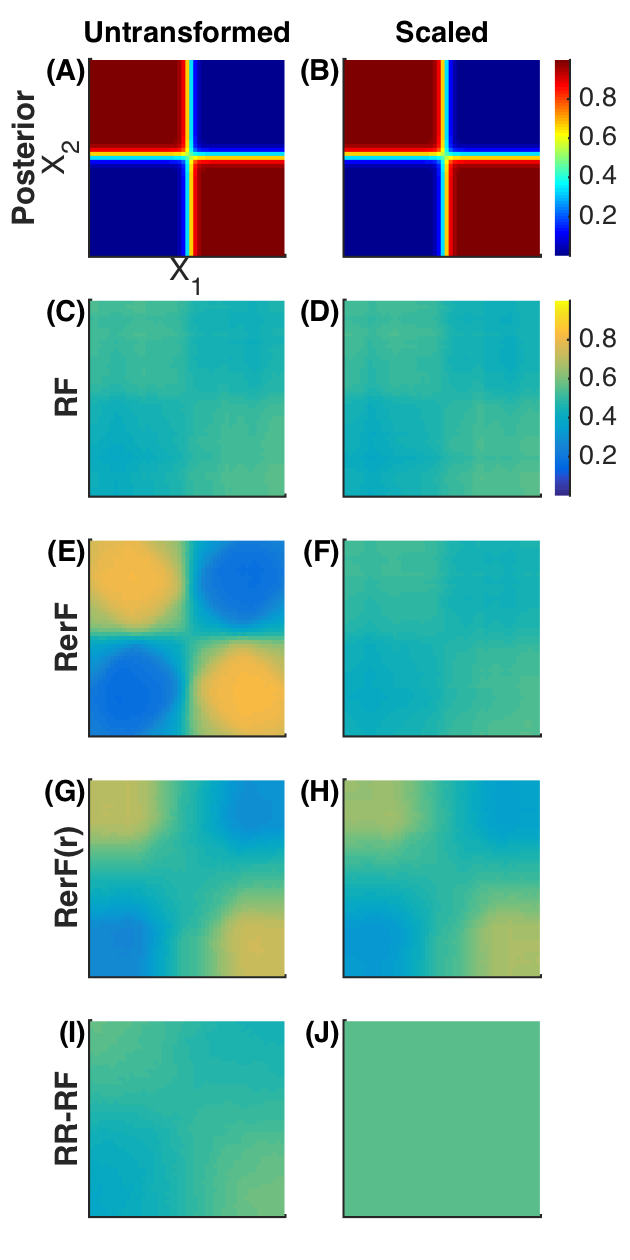
\includegraphics[width=0.38\textwidth] {Fig1_posteriors}
\caption{Posteriors and classifier estimates of posteriors for the sparse parity problem. Oblique forests are sensitive to relative scale of predictor variables, unlike RF. RerF(r), which rank transforms the data, is more robust to scale.}
\label{posteriors}
\end{center}
\end{figure}

RR-RF is an oblique decision forest method that has been recently proposed in \cite{Blaser2016}. Uniformly random rotations of the feature space imply that in general, splits will not be sparse. Therefore, we conjecture that RR-RF will perform increasingly poorly as the ratio of the number of irrelevant features to the number of relevant features becomes larger, while RF and RerF will be relatively more robust to the increasing presence of irrelevant features. Furthermore, we suspect that RR-RF will be especially sensitive to the relative scales of the predictor variables, since it is linearly combining a large number of features.

Figure \ref{posteriors} depicts both the true class posterior probabilities and estimates of the posteriors for RF, RerF, and RR-RF in two different representations of the sparse parity simulation. The left column is the native sparse parity simulation and the right column is the sparse parity simulation with dimensions randomly scaled by factors sampled uniformly from $[10^{-5},10^5]$. For this simulation, $p = 15$, $p^* = 3$, and $n = 1000$, where $p$ is the total number of dimensions, $p^*$ is the number of relevant dimensions, and n is the number of sampled data points. The number of trees used for all three algorithms was 500. Various values of $d$, the number of columns in the random projection matrix $A$, were tried and the best for each algorithm was selected. 

Comparing panels C, E, G, and I with panel A shows that RerF gives estimates of the posteriors closest to the true posteriors, followed by RerF(r). RF produces poor estimates because the linearly combinations of predictors are more informative than single predictors. RR-RF produces poor estimates because the proportion of irrelevant predictor variables is large, so that rotating the data is likely to obscure the signal. Comparing panels C and D show that RF isn't affected by scale. Comparing panel E with F and I with J show that both RerF and RR-RF are sensitive to scale. Panels G and H demonstrate that RerF(r), on the other hand, maintains ability to produce reasonable estimates of the class posteriors.

The left panels of Figure \ref{simulations} show two-dimensional scatter plots from each of the two example simulations (using the first two coordinate dimensions). The middle panels show the error rate relative to RF against the number of observed dimensions $p$. Relative error was computed as the difference between the error of either RerF, RerF(r), F-RC, and RR-RF and that of RF. The error of RF relative to itself is shown for reference. The right panels show training time against $p$ for all classifiers. The number of trees used for each method in the sparse parity and Trunk simulations were 500 and 1000, respectively. In all methods, trees were pruned and the minimum number of data points at a node in order to be considered for splitting was 10. The split criteria used was Gini impurity. The only hyperparameter tuned was $d$, the number of candidate split directions evaluated at each split node. When $p \leq 5$, each classifier was trained for all $d \in [p]$. When $p > 5$, each classifier was trained for all $d \in \{1,p^{1/4},p^{1/2},p^{3/4},p\}$ Additionally, RerF, RerF(r), and F-RC were trained for $d \in {p^{3/2},p^2}$. Note that for RF and RR-RF, $d$ is restricted to be no greater than $p$ by definition. For F-RC, the hyperparameter K, which denotes the number of predictor variables to linearly combine when forming candidate splits, was fixed to two. Errors for each classifier were selected as the lowest achieved from the different values of $d$ tried. Training times for each classifier are the average given by all values of $d$ tried. For sparse parity, $n$ was fixed at 1000 and classifiers were evaluated for $p \in \{2,5,10,25,50,100\}$. The relevant number of features $p*$ was fixed at a value of 3. For Trunk, $n$ was fixed at 100 and RF and RerF were evaluated for $p \in \{2,10,50,100,500,1000\}$. RR-RF was not evaluated for $p = 1000$ due to computational burden. Relative error and training times plotted are the average of 25 trials, and error bars represent the standard error of the mean.

In panel B, both RerF and F-RC perform as well as or better than both RF and RR-RF for all values of $p$. RerF(r) performs better than RF when $p = 10$ and performs about the same otherwise. RR-RF performs as well as or better than RF except for when $p = 25$. As conjectured, RR-RF performs better than RF when $p$ is small because oblique splits provide an advantage over axis-aligned splits in the sparse parity problem. As $p$ increases and the ratio $p^*/p$ decreases, RerF begins to outperform RR-RF. Ultimately, when this ratio is small enough, RR-RF performs even worse than RF. RerF and F-RC's ability to perform relatively well can be attributed to the sparsity of oblique splits. In panel E, RerF, RerF(r), and F-RC outperform RF for all values of $p$. This is because linear combinations of a few features can yield a higher signal-to-noise ratio than any single feature. RR-RF exhibits superior performance up to $p = 100$. RR-RF is able to perform better than RerF, RerF(r), and F-RC in these cases because a larger number of features can be linearly combined to yield an even higher signal-to-noise ratio. When $p = 500$, classification performance of RR-RF significantly degrades and exhibits the highest error rate. This can be explained by the fact that when $p$ is large enough, RR-RF often samples linear combinations of many features each having a low signal-to-noise ratio. Such projections will yield a lower signal-to-noise ratio than any single feature. In panels C and F, training times are comparable when $p$ is small. As panel F indicates, training time of RR-RF is significantly longer than the others when $p = 500$.

\begin{figure}[ht]
\vskip 0.2in
\begin{center}
\centerline{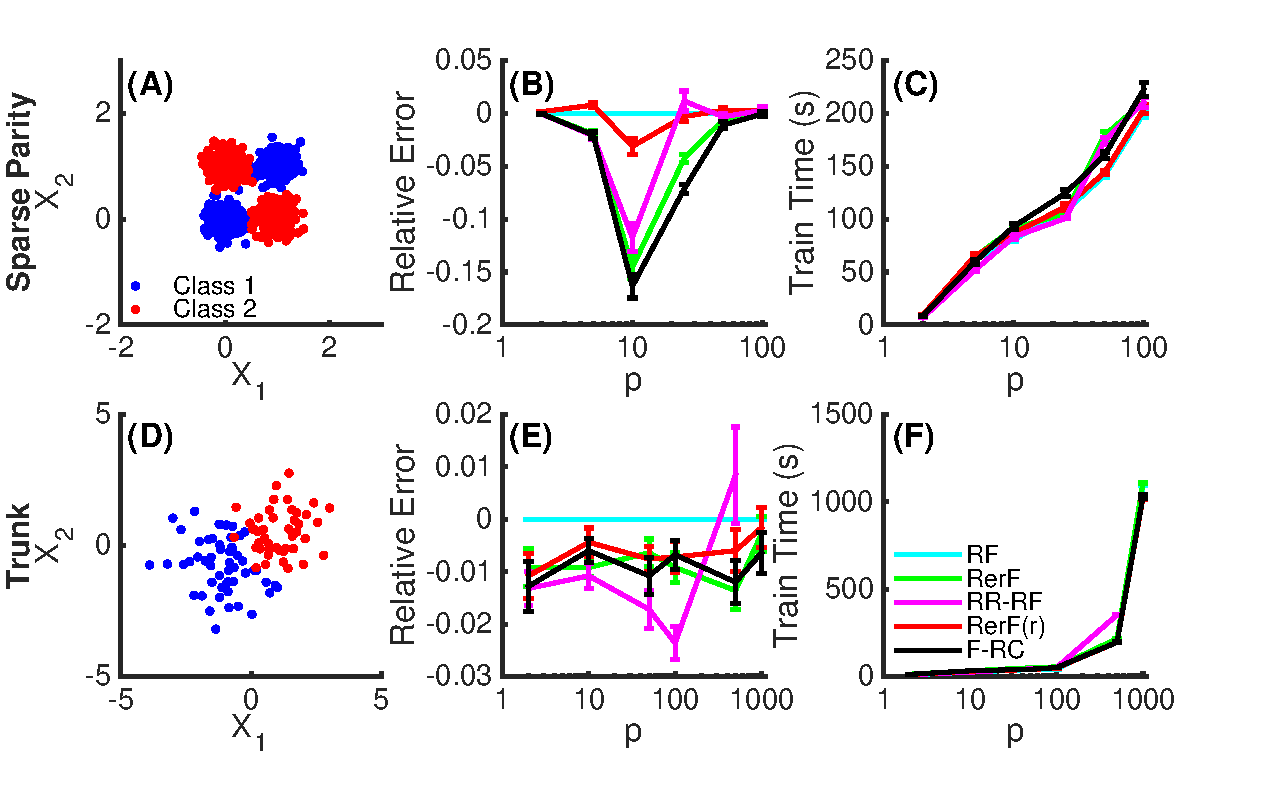
\includegraphics[width=\columnwidth]{Fig2_simulations}}
\caption{Sparse parity (A-C) and Trunk (D-F) simulations (see section \ref{section: sims} for details). (A) and (D): Scatterplots of sampled points in the first two dimensions. (B) and (E): Error rates of various random projection forest classifiers relative to RF across different values of p. (C) and (F): Same as (B) and (E) except absolute training time is plotted on the y-axis instead. All oblique methods do better than RF when the number of irrelevant features is sufficiently small, due to their ability to generate oblique parititions. However, when the number of irrelevant features becomes large enough, performance of RR-RF rapidly degrades. Training times show that RerF, RerF(r), and F-RC scales comparably with RF, while RR-RF scales poorly with large p (note that in panels E and F, RR-RF is only plotted up to $p = 500$ due to computational constraints. \emph{Note}: the color-coding here is adopted in figures \ref{transformations} and \ref{benchmark} that follow.}
\label{simulations}
\end{center}
\vskip -0.2in
\end{figure}

\subsection{Theoretical Space and Time Complexity}

For a RF, assume there are $L$ trees. If there are $m$ data points per tree, and each tree grows until terminal nodes have only $\mc O(1)$ data points with $p$ coordinates in them, there are $\mc O(m)$ nodes.
Then the complexity of constructing the random forest, disregarding cross-validation or other randomization techniques for preventing overfitting, is $\mc O(Lm^2p\log m)$. In practice the trees are shallower and stop much earlier than when nodes have $\mc O(1)$ points, so ``in practice'' the complexity often appears to be $\mc O(Lmp\log m)$. Storing RF requires $\mc{O}(L m\log m)$ because each node can be represented by the index of the nonzero coordinate. The only additional space constraint is storing which indices are positive, and which are negative, which is merely another constant.

RerF has a very similar time and space complexity, unlike many of the other oblique random forest variants.  Specifically, assume that RerF also has $L$ trees, and $m$ data points per tree, and no pruning, so $\mc O(m)$ nodes. Let $m_k$ be the number of data points at node $k$ of the tree. Like RF, RerF requires $\mc{O}(p)$ time to sample $p$ non-zero numbers, and $\mc{O}(pm_k)$ time to obtain the new matrix, $\mt{X}$, because it is a sparse matrix multiplication, in node $k$ with $\mc O(m_k)$ points. RerF also takes another $\mc{O}(p/m\log(p/m))=\mc O(1)$ time to find the best dimension. Thus, in total, in the case of well-balanced trees, RerF also requires only $\mc{O}(Lpm^2\log m)$ time to train.  To store the resulting RerF, like RF, requires $\mc{O}(L m\log m)$, because each node can be represented by the indices of the coordinates that received a non-zero element, and the expected number of such indices is $\mc O(1)$. Note that these numbers are in stark contrast to other oblique methods. RR-RFs, in particular, require a QR decomposition having a time complexity of $\mc O(p^3)$ in order to generate random rotation matrix for each tree. Rotating the data matrix prior to inducing each tree additionally requires $\mc O(mp^2)$. Therefore, RR-RF becomes very expensive to compute when $p$ is large. This can explain the trend seen in Figure \ref{simulations}(F). In addition to storing all of the decision trees, RR-RF has to store a rotation matrix for each tree, which requires $\mc O(p^2)$.

\subsection{Effects of Transformations and Outliers}
\label{section: trans}

We next want to compare the robustness classifier robustness to various data transformations across a variety of simulation settings. To do so, we consider several different modifications to the simulation settings described in the previous section: rotation, scale, affine, and outliers. To rotate the data, we simply generate rotation matrices uniformly and apply them to the data. To scale, we applied a scaling factor sampled from a uniform distribution on the interval $[10^{-5},10^5]$ to each dimension. Affine transformations were performed by applying a rotation followed by scaling as just described. Additionally, we examined the effects of introducing outliers. Outliers were introduced by sampling points from the distributions as previously described but instead using covariance matrices scaled up by a factor of four. Empirically, an addition of 20 points from these outlier models to the original 100 points was found to produce a noticeable but not overwhelming effect on classifier performance.

Figure \ref{transformations} shows the effect of these transformations and outliers on the sparse parity (panels A-E) and Trunk (panels F-J) problems. Comparing panel B with A shows that all methods except for RR-RF and RF are affected by rotations, by noting that their error rates are noticeably shifted up for $p \geq 25$. Comparing panel G with F shows that when $p = 500$ all classifiers except for RR-RF incur a loss in performance when the data is rotated. Comparing panel C with A and panel H with F show that F-RC and RR-RF suffer an increase in error rate when the data is  scaled (error rate of RR-RF in panel H exceeds the y-axis limits), RerF is slightly hurt, and RerF(r) and RF are unaffected. In panels D and I, all classifiers are sensitive to affine transformations. However, RerF is more robust than F-RC and RR-RF, and RerF(r) is even more robust. Panels E and J show that all methods are slightly affected by the introduction of outliers. 

\begin{figure}[ht]
\vskip 0.2in
\begin{center}
\centerline{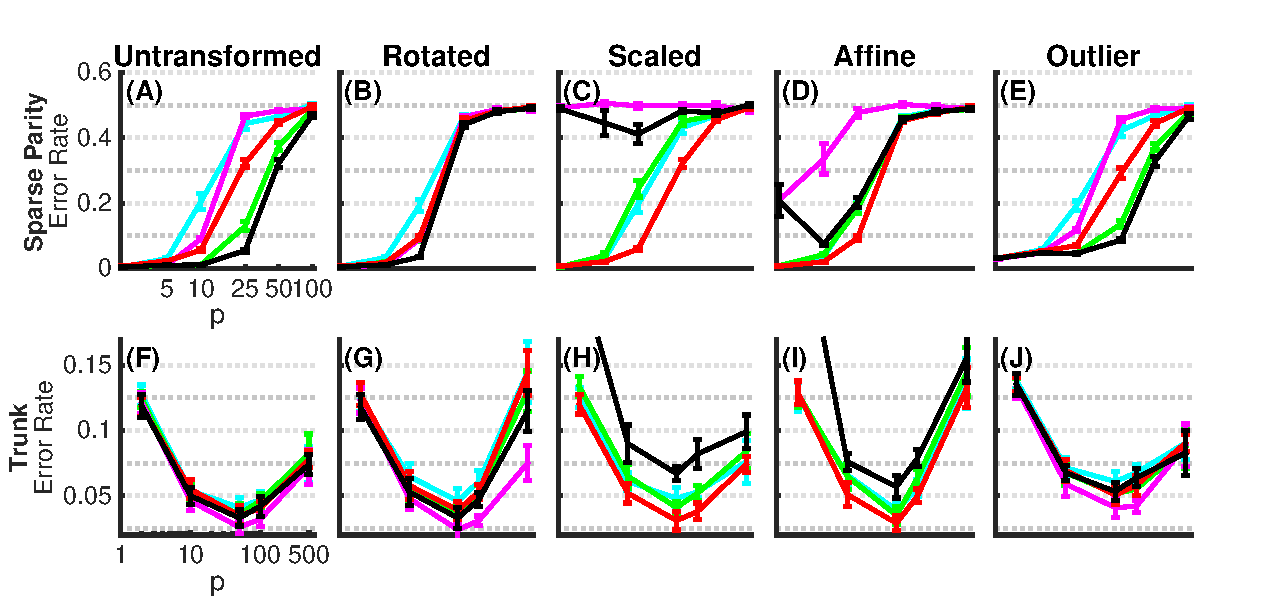
\includegraphics[width=\columnwidth]{Fig3_transformations2}}
\caption{The effects of different transformations applied to the sparse parity (A-E) and Trunk (F-J) simulations on classification performance (see section \ref{section: trans} for details). Specifically, we consider rotations, scalings, affine transformations, as well as the addition of outliers. RR-RF and F-RC are severely affected by random scaling of the predictor variables, and therefore, also affected by affine transformations. RerF is slightly affected by scale, while RerF(r) is unaffected. When a general affine transformation is applied, RerF(r) is the most robust.}
\label{transformations}
\end{center}
\vskip -0.2in
\end{figure}

\subsection{Benchmark Data}
\label{section: benchmark}

In addition to the simulations, RF, RerF, F-RC, and RR-RF were evaluated on 113 of the 121 datasets as described in \cite{Delgado2014}. The eight remaining datasets were not used because their high dimensionality and large number of data points rendered the classifiers both time and space costly, particularly for RR-RF. As in the previous section, transformations, with the exception of outliers, were applied to the datasets to observe their affects on performance of the three algorithms. Classifiers were trained on the entire training sets provided. For each data set, error rates were again estimated by out of bag error. The number of trees used in each algorithm was 1000 for datasets having at most 1000 data points and 500 for datasets having greater than 1000 data points. When $p \leq 5$, each algorithm was trained for all $d \in [p]$. When $p > 5$, each algorithm was trained for all $d \in \{1,p^{1/4},p^{1/2},p^{3/4},p\}$. Error rates for each algorithm were selected as the minimum given by the five. For each dataset, relative performance ratios for each algorithm were computed by dividing the error rate of each algorithm by the minimum error rate of the three. The empirical cumulative distribution functions of relative performance ratios for each algorithm were computed and plotted in Figure \ref{benchmark}. Such plots are called performance profiles \cite{Dolan2002}. Performance profiles are useful in visualizing how frequently a particular algorithm wins, and when it loses, how frequently it loses by a certain amount. For instance, a value of 0.9 on the y-axis and a value of 2.0 on the x-axis means that the error of that classifier was at most twice the error of the best performing classifier on a given dataset in 90$\%$ of all benchmark datasets. 

In panel A of Figure \ref{benchmark}, F-RC, RerF, and RerF(r) outperform RF, while RR-RF exhibits inferior performance. Panel B shows that when the benchmark datasets are rotated, RR-RF and F-RC perform the best, followed by RerF and RerF(r), and lastly RF. Panel C shows that RerF(r) performs the best when the predictors are randomly scaled, while RF, RerF, and F-RC are approximately the same. Lastly, panel D shows that RerF(r) performs the best when affine transformations are applied, while F-RC and RR-RF perform very poorly. 

\begin{figure}[ht]
\vskip 0.2in
\begin{center}
\centerline{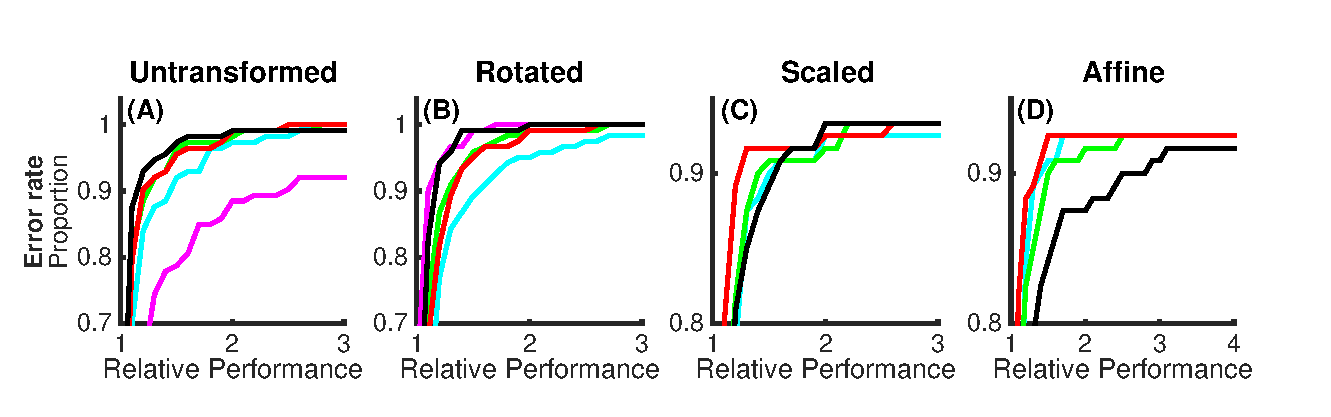
\includegraphics[width=\columnwidth]{Fig4_benchmark}}
\caption{Classification performance profiles on benchmarks with various transformations applied (see section \ref{section: benchmark} for details). In terms of classification accuracy, RerF performs as well as or better than RF in all settings except for when affine transformations are applied to the data. RerF, RerF(r), and F-RC outperform RR-RF for all settings except for when the data is rotated. RR-RF performs terribly when scale or affine transformations are applied, and F-RC also performs poorly when affine transformations are applied. RerF(r) dominates all others in the face of affine transformations.}
\label{benchmark}
\end{center}
\vskip -0.2in
\end{figure}

\section{Conclusion and Future Work}

We have proposed novel methods for constructing decision forests, which we call RerFs. We view these methods as special cases of a more general random projection forest, which include Breiman's original Forest-RI and Forest-RC, as well as previously proposed oblique decision forests. Our proposed method bares some similarity to Forest-RC, but is different in important ways. The choice of $f_A(\mc{D}_l)$ we propose produces a decision forest that is more computationally efficient. Additionally, it can be viewed as a generalization of both RF and F-RC by noting that we don't restrict the number of nonzeros per column to be fixed across A. Instead, we have columns of varying sparsity. This imparts more diversity into the decision forest and can enhance performance. We have demonstrated in simulations that RerFs are especially well-suited for classification problems in which axis-parallel splits are suboptimal, and at the same time, have a large number of irrelevant features relative to relevant ones. This could explain RerF's excellent empirical performance on a suite of 113 benchmark datasets, as real data often has the properties just described. Moreover, RerF preserves the time and space complexity of Forest-RI, and is more robust to affine transformations than are other oblique methods, especially the variant RerF(r).

The simplicity of RerFs and the nice properties of very sparse random projections \cite{Li2006} suggest that they will be amenable to theoretical investigation, extending the work of Scornet et al. (2015) to the RerF setting \cite{Scornet2015}. Moreover, we hope that theoretical investigations will yield more insight into which distributions $f_A(\mc{D}_l)$ will be optimal under different distributional settings, both asymptotically and under finite sample assumptions. Even under the currently proposed $f_A(\mc{D}_l)$, our implementation has room for improvement. Although it has the same space and time complexity as RF, we will determine explicit constants, and improve our implementation accordingly. Indeed, our current implementation is a proof-of-concept MATLAB implementation. We will utilize recent GPU and semi-external memory methods to significantly speed up RerF \cite{zheng15flashgraph}. As with all decision forests, multiclass classification is but one exploitation task they can be used for; therefore, we will also extend this work to enable regression, density estimation, clustering, and hashing. We will provide open source code to enable more rigorous and extended analyses by the machine learning community.

\bibliography{aaai17_robust_oblique_forests.bib}
\bibliographystyle{aaai}

\end{document}
